\section{Simulink Model and Validation Suite}
\label{app:simulink}
The validation suite (\code{shuffler\_string\_validate.m}) runs seven tests on the MIL model (4 modules, 3 shufflers, $k=1$, cold start) and the first five on the carpark twin (3 modules, 2 shufflers, sensing model). Pass criteria: settled ($|\Delta\vd| < 0.05\V$, $|\Delta\ic| < 0.5\A$ between two 10\,ms windows), track ($|\vd - r_v| < 0.25\V$, $|\ic| < 1\A$), MPPT (module power above 98.5\,\% of the per-module ceiling) and protect ($|\ic| < 1\A$, $|i_{diff}| \le 10\A$). \Cref{fig:mil_validate} shows one tracking test and the protection test as examples; every test's figures are regenerated by the script and are in \code{8\_Results/analysis/out/figures/}.

\begin{table}[htbp]\centering\scriptsize
\caption{Validate test matrix.}
\label{tab:validate}
\begin{tabular}{l l p{2.6cm} p{2.6cm} l l p{2.6cm}}
\toprule
\# & Test & irradiance on the shaded module & $r_v$ & $T_{stop}$ & mode & result (MIL / carpark)\\
\midrule
01 & uniform-zero & 1000\,W/m$^2$ & 0 & 0.06\,s & track & PASS / PASS\\
02 & decoupling & 1000 & $[0\;2\;0]$ (carpark $[0\;2]$) & 0.06 & track & PASS / PASS\\
03 & shade-balanced & 500 & 0 & 0.06 & track & PASS / PASS\\
04 & shade-refs & 500 & $[0\;2\;-2]$ (carpark $[2\;-2]$) & 0.06 & track & PASS / PASS\\
05 & shade-deep & 200 & 0 & 0.50 & protect & PASS / PASS\\
06 & mppt-uniform & 1000 & 0 & 0.60 & mppt & PASS / (CC load only)\\
07 & mppt-shade & 500 & 0 & 0.60 & mppt & PASS / (CC load only)\\
\bottomrule
\end{tabular}
\end{table}

\begin{figure}[htbp]
  \centering
  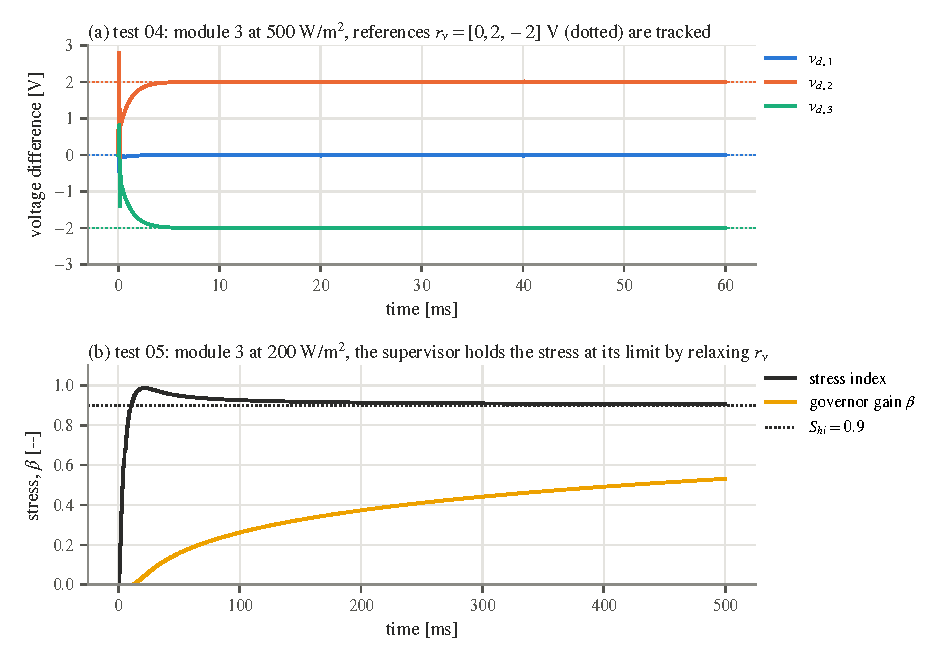
\includegraphics[width=\linewidth]{results/mil_validate}
  \caption[{Two of the MIL validation tests}]{Two of the MIL validation tests: (a) tracking non-zero references under shade, (b) deep shade, where the feasibility governor raises $\beta$ to relax the references and keep the shuffler inside its current rating.}
  \label{fig:mil_validate}
\end{figure}

\begin{figure}[htbp]
  \centering
  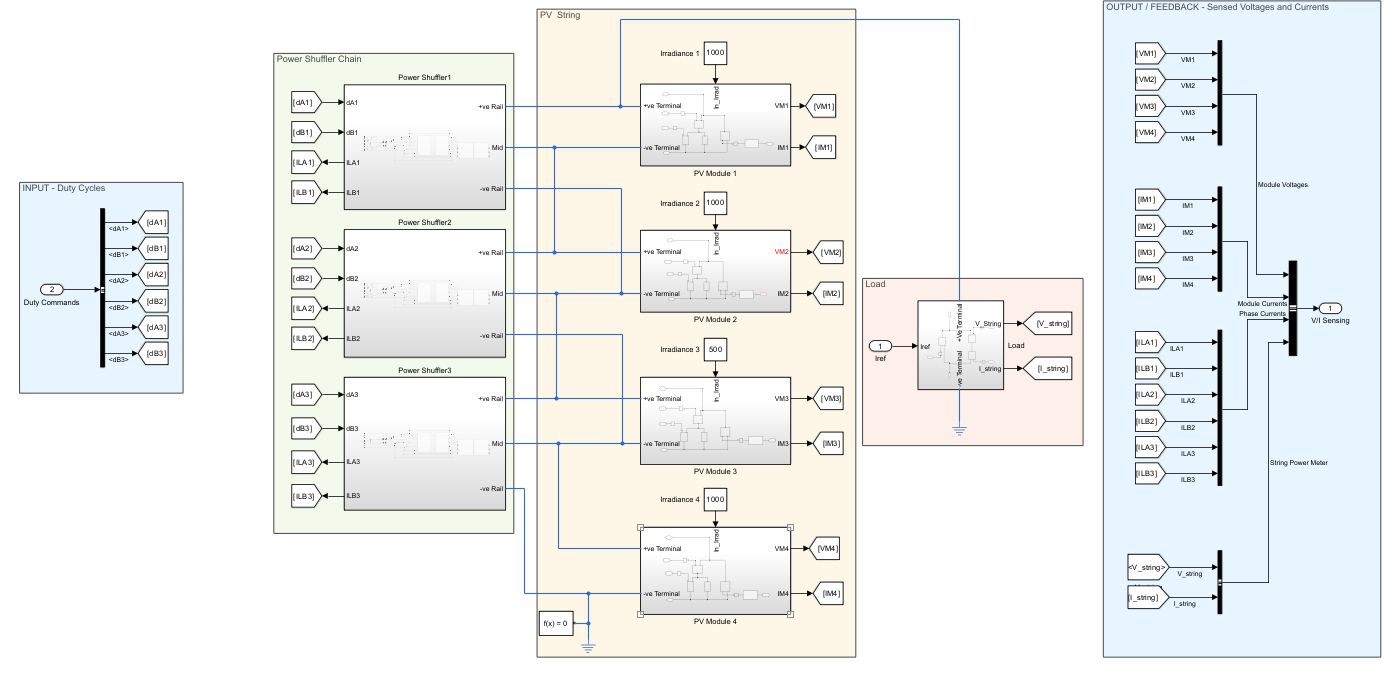
\includegraphics[width=0.92\linewidth]{img-014-016}
  \caption{Inside the MIL plant: four AIKO-class modules and three averaged-switch shufflers.}
  \label{fig:mil_plant}
\end{figure}

\begin{figure}[htbp]
  \centering
  \begin{subfigure}[t]{\linewidth}\centering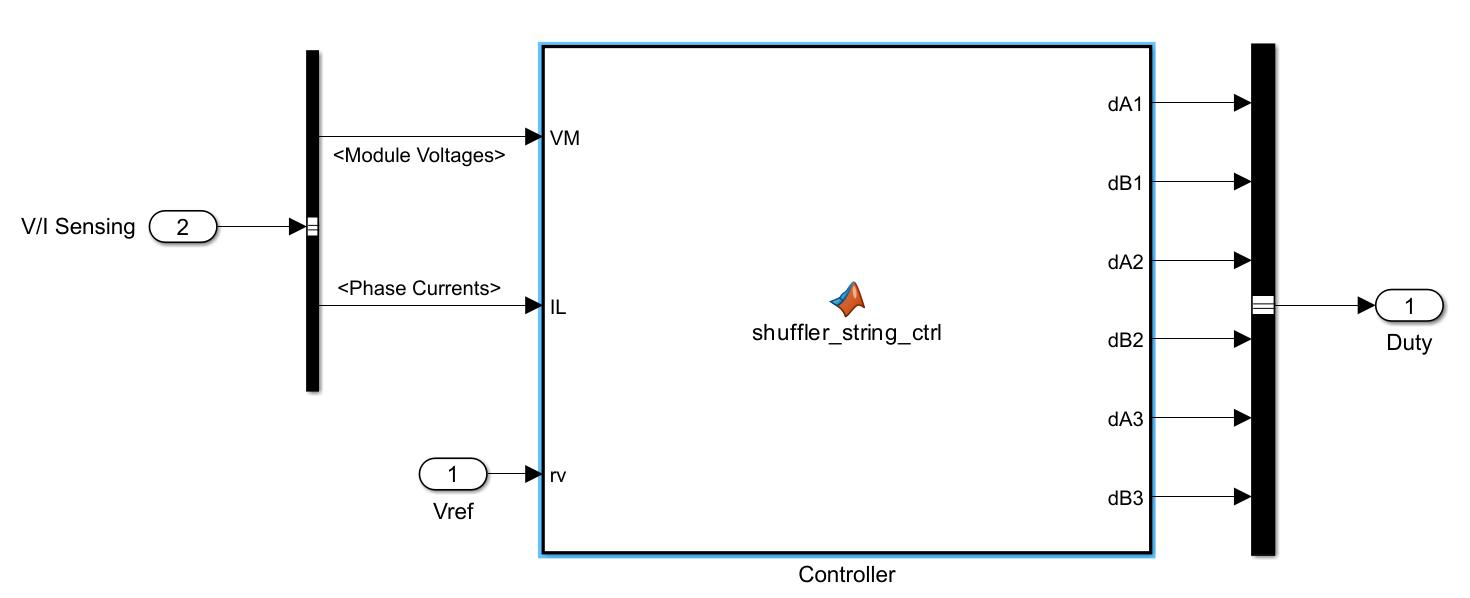
\includegraphics[width=0.9\linewidth]{img-015-017}\caption{Controller block.}\end{subfigure}\\[6pt]
  \begin{subfigure}[t]{\linewidth}\centering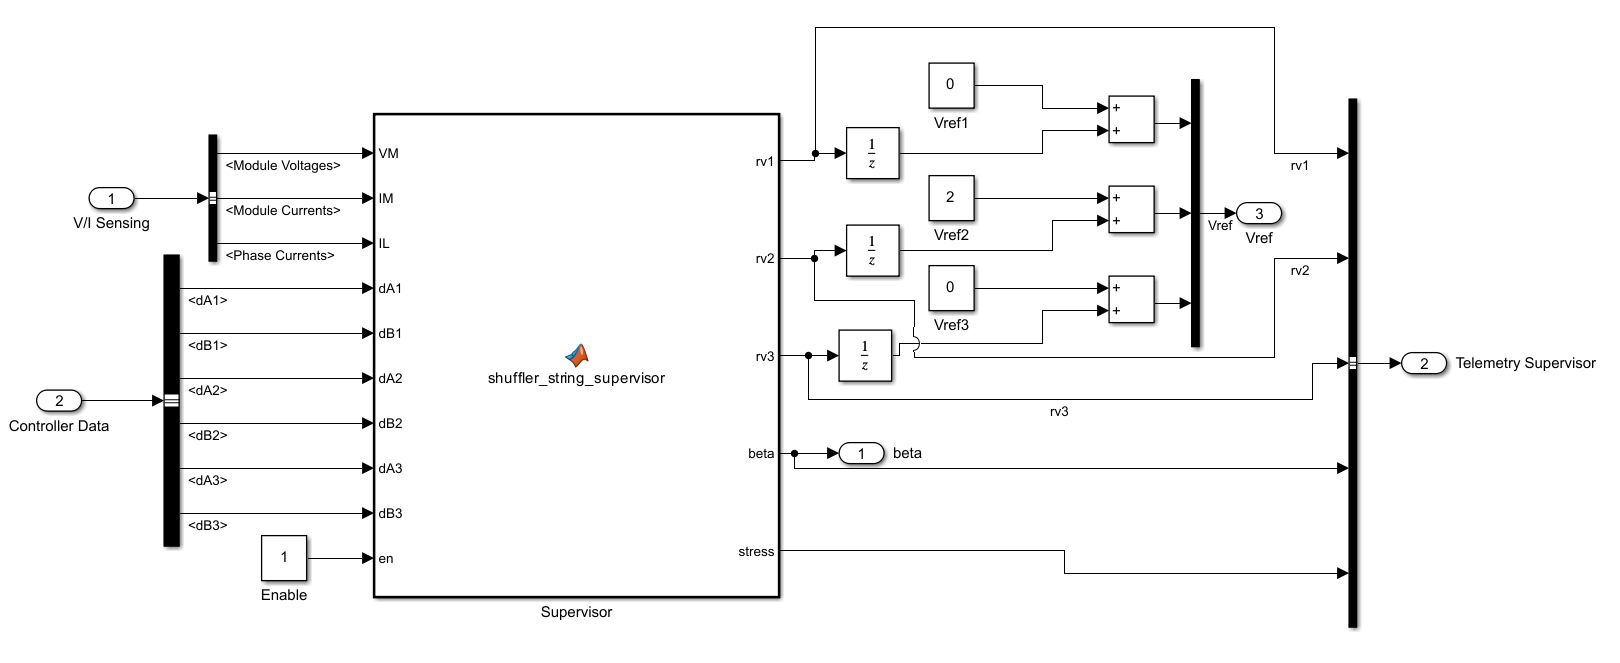
\includegraphics[width=0.9\linewidth]{img-015-018}\caption{Supervisor block.}\end{subfigure}\\[6pt]
  \begin{subfigure}[t]{\linewidth}\centering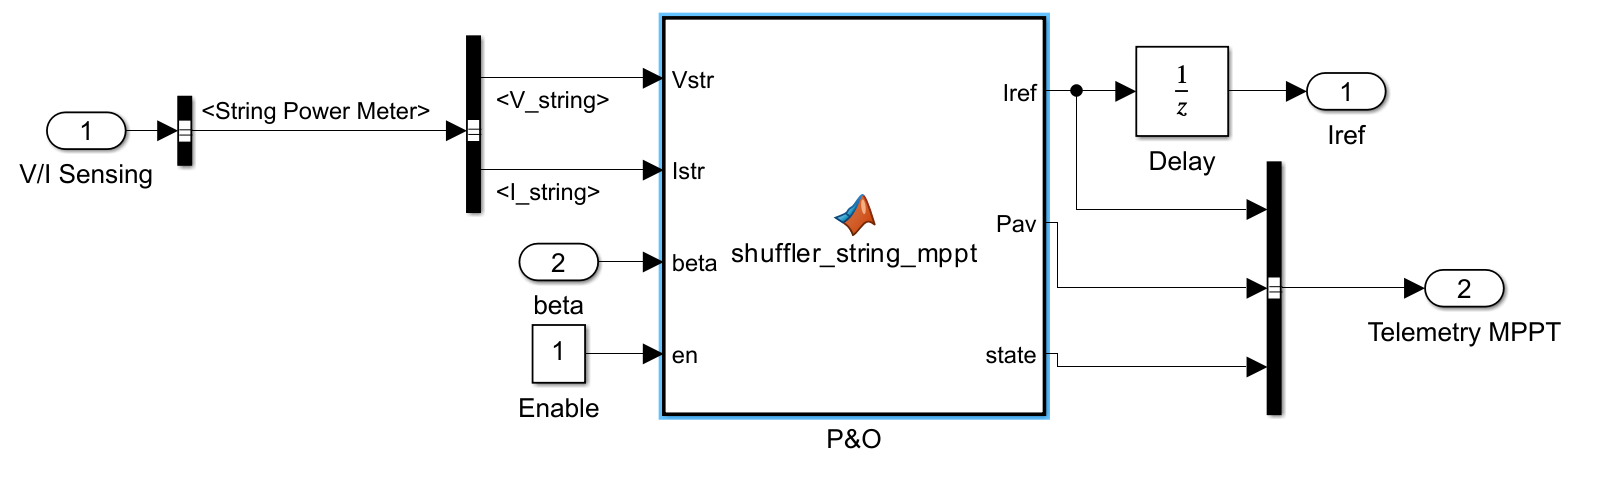
\includegraphics[width=0.9\linewidth]{img-015-019}\caption{MPPT (P\&O) block.}\end{subfigure}
  \caption[{Controller, supervisor and MPPT blocks of the Simulink MIL model}]{The controller, supervisor and MPPT blocks of the Simulink MIL model (\cref{fig:mil}).}
  \label{fig:mil_blocks}
\end{figure}
